%%%%%%%%%%%%%%%%%%%%%%%%%%%%%%%%%%%%%%%%%
% Programming/Coding Assignment
% LaTeX Template
%
% This template has been downloaded from:
% http://www.latextemplates.com
%
% Original author:
% Ted Pavlic (http://www.tedpavlic.com)
%
% Note:
% The \lipsum[#] commands throughout this template generate dummy text
% to fill the template out. These commands should all be removed when 
% writing assignment content.
%
% This template uses a Perl script as an example snippet of code, most other
% languages are also usable. Configure them in the "CODE INCLUSION 
% CONFIGURATION" section.
%
%%%%%%%%%%%%%%%%%%%%%%%%%%%%%%%%%%%%%%%%%

%----------------------------------------------------------------------------------------
%	PACKAGES AND OTHER DOCUMENT CONFIGURATIONS
%----------------------------------------------------------------------------------------

\documentclass{article}

\usepackage{fancyhdr} % Required for custom headers
\usepackage{lastpage} % Required to determine the last page for the footer
\usepackage{extramarks} % Required for headers and footers
\usepackage[usenames,dvipsnames]{color} % Required for custom colors
\usepackage{graphicx} % Required to insert images
\usepackage{listings} % Required for insertion of code
\usepackage{courier} % Required for the courier font
\usepackage{lipsum} % Used for inserting dummy 'Lorem ipsum' text into the template
\usepackage{amsmath}
\usepackage{booktabs}
\usepackage{bigstrut}
\usepackage{float}
\usepackage{hyperref}
\usepackage{color}

\hypersetup{
    colorlinks   = true,    % Colours links instead of ugly boxes
    urlcolor     = red,    % Colour for external hyperlinks
    linkcolor    = red,    % Colour of internal links
    citecolor    = red      % Colour of citations
}
% Margins
\topmargin=-0.45in
\evensidemargin=0in
\oddsidemargin=0in
\textwidth=6.5in
\textheight=9.0in
\headsep=0.25in

\linespread{1.1} % Line spacing

% Set up the header and footer
\pagestyle{fancy}
\lhead{\hmwkAuthorName} % Top left header
\chead{\hmwkClass\ : \hmwkTitle} % Top center head
\rhead{\firstxmark} % Top right header
\lfoot{\lastxmark} % Bottom left footer
\cfoot{} % Bottom center footer
\rfoot{Page\ \thepage\ of\ \protect\pageref{LastPage}} % Bottom right footer
\renewcommand\headrulewidth{0.4pt} % Size of the header rule
\renewcommand\footrulewidth{0.4pt} % Size of the footer rule

\setlength\parindent{0pt} % Removes all indentation from paragraphs

%----------------------------------------------------------------------------------------
%	CODE INCLUSION CONFIGURATION
%----------------------------------------------------------------------------------------

\definecolor{MyDarkGreen}{rgb}{0.0,0.4,0.0} % This is the color used for comments
\lstloadlanguages{Perl} % Load Perl syntax for listings, for a list of other languages supported see: ftp://ftp.tex.ac.uk/tex-archive/macros/latex/contrib/listings/listings.pdf
\lstset{language=Perl, % Use Perl in this example
    frame=single, % Single frame around code
    basicstyle=\small\ttfamily, % Use small true type font
    keywordstyle=[1]\color{Blue}\bf, % Perl functions bold and blue
    keywordstyle=[2]\color{Purple}, % Perl function arguments purple
    keywordstyle=[3]\color{Blue}\underbar, % Custom functions underlined and blue
    identifierstyle=, % Nothing special about identifiers                                         
    commentstyle=\usefont{T1}{pcr}{m}{sl}\color{MyDarkGreen}\small, % Comments small dark green courier font
    stringstyle=\color{Purple}, % Strings are purple
    showstringspaces=false, % Don't put marks in string spaces
    tabsize=5, % 5 spaces per tab
    %
    % Put standard Perl functions not included in the default language here
    morekeywords={rand},
    %
    % Put Perl function parameters here
    morekeywords=[2]{on, off, interp},
    %
    % Put user defined functions here
    morekeywords=[3]{test},
    %
    morecomment=[l][\color{Blue}]{...}, % Line continuation (...) like blue comment
    numbers=left, % Line numbers on left
    firstnumber=1, % Line numbers start with line 1
    numberstyle=\tiny\color{Blue}, % Line numbers are blue and small
    stepnumber=5 % Line numbers go in steps of 5
}

% Creates a new command to include a perl script, the first parameter is the filename of the script (without .pl), the second parameter is the caption
\newcommand{\perlscript}[2]{
    \begin{itemize}
        \item[]\lstinputlisting[caption=#2,label=#1]{#1.py}
    \end{itemize}
}
\newcommand{\cppscript}[2]{
    \begin{itemize}
        \item[]\lstinputlisting[]{#1}
    \end{itemize}
}

%----------------------------------------------------------------------------------------
%	DOCUMENT STRUCTURE COMMANDS
%	Skip this unless you know what you're doing
%----------------------------------------------------------------------------------------

% Header and footer for when a page split occurs within a problem environment
\newcommand{\enterProblemHeader}[1]{
    \nobreak\extramarks{#1}{#1 continued on next page\ldots}\nobreak
    \nobreak\extramarks{#1 (continued)}{#1 continued on next page\ldots}\nobreak
}

% Header and footer for when a page split occurs between problem environments
\newcommand{\exitProblemHeader}[1]{
    \nobreak\extramarks{#1 (continued)}{#1 continued on next page\ldots}\nobreak
    \nobreak\extramarks{#1}{}\nobreak
}

%\setcounter{secnumdepth}{0} % Removes default section numbers
\newcounter{homeworkProblemCounter} % Creates a counter to keep track of the number of problems

\newcommand{\homeworkProblemName}{}
\newenvironment{homeworkProblem}[1][Problem \arabic{homeworkProblemCounter}]{ % Makes a new environment called homeworkProblem which takes 1 argument (custom name) but the default is "Problem #"
    \stepcounter{homeworkProblemCounter} % Increase counter for number of problems
    \renewcommand{\homeworkProblemName}{#1} % Assign \homeworkProblemName the name of the problem
    \section{\homeworkProblemName} % Make a section in the document with the custom problem count
    \enterProblemHeader{\homeworkProblemName} % Header and footer within the environment
    }{
    \exitProblemHeader{\homeworkProblemName} % Header and footer after the environment
}

\newcommand{\problemAnswer}[1]{ % Defines the problem answer command with the content as the only argument
\noindent\framebox[\columnwidth][c]{\begin{minipage}{0.98\columnwidth}#1\end{minipage}} % Makes the box around the problem answer and puts the content inside
}

\newcommand{\homeworkSectionName}{}
\newenvironment{homeworkSection}[1]{ % New environment for sections within homework problems, takes 1 argument - the name of the section
    \renewcommand{\homeworkSectionName}{#1} % Assign \homeworkSectionName to the name of the section from the environment argument
    \subsection{\homeworkSectionName} % Make a subsection with the custom name of the subsection
    \enterProblemHeader{\homeworkProblemName\ [\homeworkSectionName]} % Header and footer within the environment
    }{
    \enterProblemHeader{\homeworkProblemName} % Header and footer after the environment
}

%----------------------------------------------------------------------------------------
%	NAME AND CLASS SECTION
%----------------------------------------------------------------------------------------

\newcommand{\hmwkTitle}{homework 01} % Assignment title
\newcommand{\hmwkDueDate}{Tuesday,\ Febrary\ 28,\ 2017} % Due date
\newcommand{\hmwkClass}{Numerical Analysis} % Course/class
\newcommand{\hmwkClassTime}{10:30am} % Class/lecture time
\newcommand{\hmwkClassInstructor}{Jones} % Teacher/lecturer
\newcommand{\hmwkAuthorName}{102061149 Fu-En Wang} % Your name

%----------------------------------------------------------------------------------------
%	TITLE PAGE
%----------------------------------------------------------------------------------------

\title{
    \vspace{2in}
    \textmd{\textbf{\hmwkClass:\ \hmwkTitle}}\\
    \normalsize\vspace{0.1in}\small{Due\ on\ \hmwkDueDate}\\
    \vspace{3in}
}

\author{\textbf{\hmwkAuthorName}}
\date{} % Insert date here if you want it to appear below your name

%----------------------------------------------------------------------------------------

\begin{document}

\maketitle

%----------------------------------------------------------------------------------------
%	TABLE OF CONTENTS
%----------------------------------------------------------------------------------------

%\setcounter{tocdepth}{1} % Uncomment this line if you don't want subsections listed in the ToC

\newpage
%\tableofcontents
%\newpage

%----------------------------------------------------------------------------------------
%	PROBLEM 1
%----------------------------------------------------------------------------------------

% To have just one problem per page, simply put a \clearpage after each problem
\section{Introduction}
When we are given an n x n squre matrix $A$, then an n x n orthogonal matrix $G$ can also be found by Gram-Schmidt process. \newline
\subsection{Gram-Schmidt process}
When \newline
\begin{gather}
A = \begin{bmatrix}A_1 & A_2 & ...... & A_n \end{bmatrix}
\end{gather}
and \newline
\begin{gather}
G = \begin{bmatrix}G_1 & G_2 & ...... & G_n\end{bmatrix}
\end{gather}

Each $A_i$ and $G_i$ is a column of squre matrix $A$ and $G$, respectively. And the algorithm of \textbf{Gram-Schmidt process} is as the
following: \newline
\begin{gather}
    G_1 = A_1 \\
    G_k = A_k - \sum_{i=1}^{k-1}{\frac{(A_k^TG_i)G_i}{G_i^TG_i}}
\end{gather}


\subsection{Sigma calculation}
Because $G$ is an orthogonal matrix, so $M = G^TG$ will be a diagonal matrix; in other words, each non-diagonal element \newline
\begin{gather}
    M[i][j], i \neq j
\end{gather}
has to be zero. To prove this property, we calculate the error of non-diagonal elements by Sigma: \newline
\begin{gather}
    \sigma = \sqrt{\sum_{i=1}^{n}\sum_{j=1,i \neq j}^{n}d_{i,j}^2}
\end{gather}
Theorectically, $\sigma$ should be very closed to zeros. \newline \newline

In this homework, we will implement three algorithms to compare their runtime.
\newpage

\section{C$++$ Implementation}
\subsection{Algorithm-1}
\cppscript{src/algo1.cpp}{algo1 implementation}
This is the most straightforward method for \textbf{Gram-Schmidt process}. In the innermost for-loop, we calculate
$\sum_{i=1}^{k-1}{\frac{(A_k^TG_i)G_i}{G_i^TG_i}}$ first and subtracted by $A[k]$, and then replace $G[k]$ by the final vector. \newline

\subsection{Algorithm-2}
\cppscript{src/algo2.cpp}{algo2 implementation}
Algo2 simplifies algo1 by modifying three terms and removing $G[k]$ = $A[k]$ - $G[k]$. And there is one more subtraction in algo1 
than algo2.

\subsection{Algorithm-3}
\cppscript{src/algo3.cpp}{algo3 implementation}
\newpage
Compared to algo2, algo3 only move the multiplication of $(G_k^TG_i)$ and $G_i$ to the last position. By such manipulation, two problems
show up:
\begin{enumerate}
    \item Will the result change? (observed by \boldmath$\sigma$) \\
    \item Will the speed change? (observed by \textbf{RUNTIME})
\end{enumerate}
We will discuss these two questions in Discussion part.

\subsection{Complexity}
Because in the innermost for-loop, we have to do $\frac{n(n+1)}{2}$; but we still need to do vector operation one time, so it will
become $n * \frac{n(n+1)}{2}$, which is a \boldmath$O(n^3)$ problem.

\section{Discussion}
\subsection{Performance Evaluation}
In this project, we focus on two numbers for performance:
\begin{enumerate}
    \item \boldmath$\sigma$ (accuracy) \\
    \item \textbf{RUNTIME} (speed)
\end{enumerate}

$\sigma$ can be regarded as the loss or error of our system, so we must make it small as possible as we can. As for RUNTIME, there are
two way to deal with it.
\begin{enumerate}
    \item Total runtime (total time of execution) \\
    \item Algorithm runtime (total time of algorithm part)
\end{enumerate}
Because total runtime consists of the time that program parses the \textbf{mX.dat}; when the matrix dimension is large, it will consume
much more time. But what we really care about is the time our algorithms consume, so I also track the algorithm time in each 
experiment. In the following part, \textbf{algo-time} is refered as algorithm runtime(seconds), 
while \textbf{runtime} refered as total runtime(seconds).


\subsection{Algorithm-1 Perormance}
Table [\ref{tab:algo1}] show detail results of algorithm-1.
\begin{table}[h!]
    \centering
    \caption{Algorithm-1 performance}
    \begin{tabular}{|c|c|c|c|c|}
        \hline
        \textbf{algo1} & n   & sigma & algo-time(s) & runrime(s) \bigstrut\\
        \hline
        m3  & 3   & 4.40E-15 & 4.05E-06 & 0.004 \bigstrut\\
        \hline
        m4  & 10  & 3.06E-13 & 2.79E-05 & 0.005 \bigstrut\\
        \hline
        m5  & 100 & 293.881 & 0.0118849 & 0.04 \bigstrut\\
        \hline
        m6  & 200 & 477.474 & 0.042047 & 0.112 \bigstrut\\
        \hline
        m7  & 400 & 717.106 & 0.242979 & 0.634 \bigstrut\\
        \hline
        m8  & 800 & 1069.88 & 1.92496 & 6.629 \bigstrut\\
        \hline
        m9  & 1600 & 1531.34 & 14.5427 & 55.245 \bigstrut\\
        \hline
    \end{tabular}%

    \label{tab:algo1}
\end{table}%
\subsubsection{Sigma}
\label{sec:algo1-sigma}
When $n$ is large, it seems that algorithm-1 get a large $\sigma$; in other words, it is not \textbf{accurate}. By my observation,
because the \textbf{magnitude} difference between $A[k]$ and $G[k]$ could be large, so the calculation error of $G[k] = A[k] - G[k]$
will be amplified, and that's why we get a large \boldmath$\sigma$
\newpage
\subsubsection{$n^3$ and runtime}
Because it is a $O(n^3)$ problem, so $n^3$ and runtime shoule be a straight line, shown by fig [\ref{fig:algo1-runtime}].
\begin{figure}[H]
    \centering
    \caption{runtime to $n^3$}
    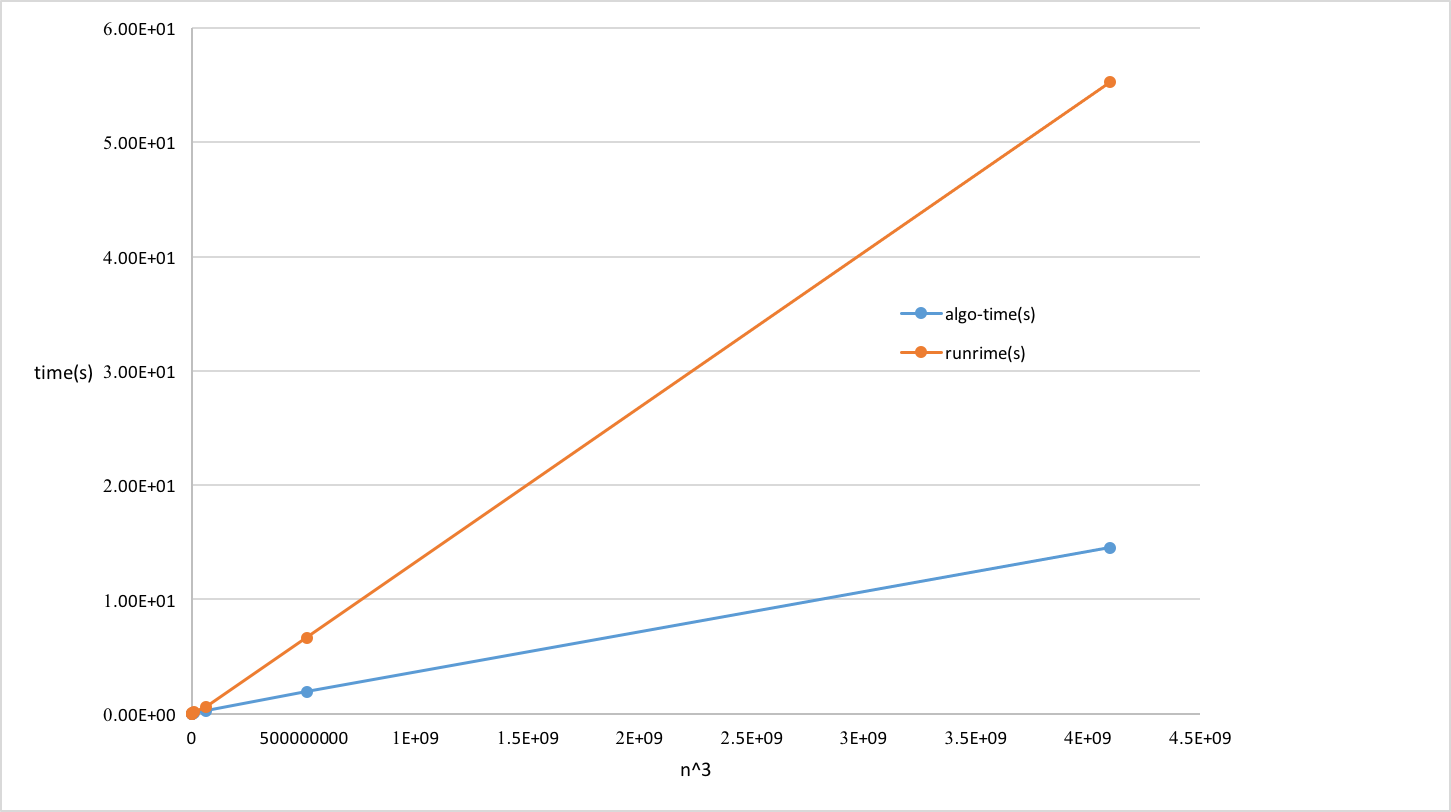
\includegraphics[width=0.75\textwidth]{src/algo1-runtime.png}
    \label{fig:algo1-runtime}
\end{figure}

\subsection{Algorithm-2 performance}
% Table generated by Excel2LaTeX from sheet '工作表1'
Table [\ref{tab:algo2}] shows detail result of Algorithm-2
\begin{table}[h]
    \centering
    \caption{Algorithm-2 performance}
    \begin{tabular}{|c|c|c|c|c|}
        \hline
        \textbf{algo2} & \multicolumn{1}{c|}{n} & \multicolumn{1}{c|}{sigma} & \multicolumn{1}{c|}{algo-time(s)} & \multicolumn{1}{c|}{runrime(s)} \bigstrut\\
        \hline
        m3  & 3   & 3.78E-15 & 4.05E-06 & 0.004 \bigstrut\\
        \hline
        m4  & 10  & 1.29E-14 & 4.91E-05 & 0.009 \bigstrut\\
        \hline
        m5  & 100 & 1.92E-13 & 0.00610399 & 0.017 \bigstrut\\
        \hline
        m6  & 200 & 6.41E-13 & 0.039006 & 0.113 \bigstrut\\
        \hline
        m7  & 400 & 2.29E-12 & 0.25009 & 0.663 \bigstrut\\
        \hline
        m8  & 800 & 9.10E-12 & 1.84492 & 6.382 \bigstrut\\
        \hline
        m9  & 1600 & 3.40E-11 & 18.2445 & 59.626 \bigstrut\\
        \hline
    \end{tabular}%

    \label{tab:algo2}
\end{table}%
\subsubsection{Sigma}
Although when n is getting larger, we will also get larger $\sigma$, but the slope $\sigma$ grows is much smaller than Algorithm-1.
\subsubsection{runtime to $n^3$}
\begin{figure}[H]
    \centering
    \caption{runtime to $n^3$}
    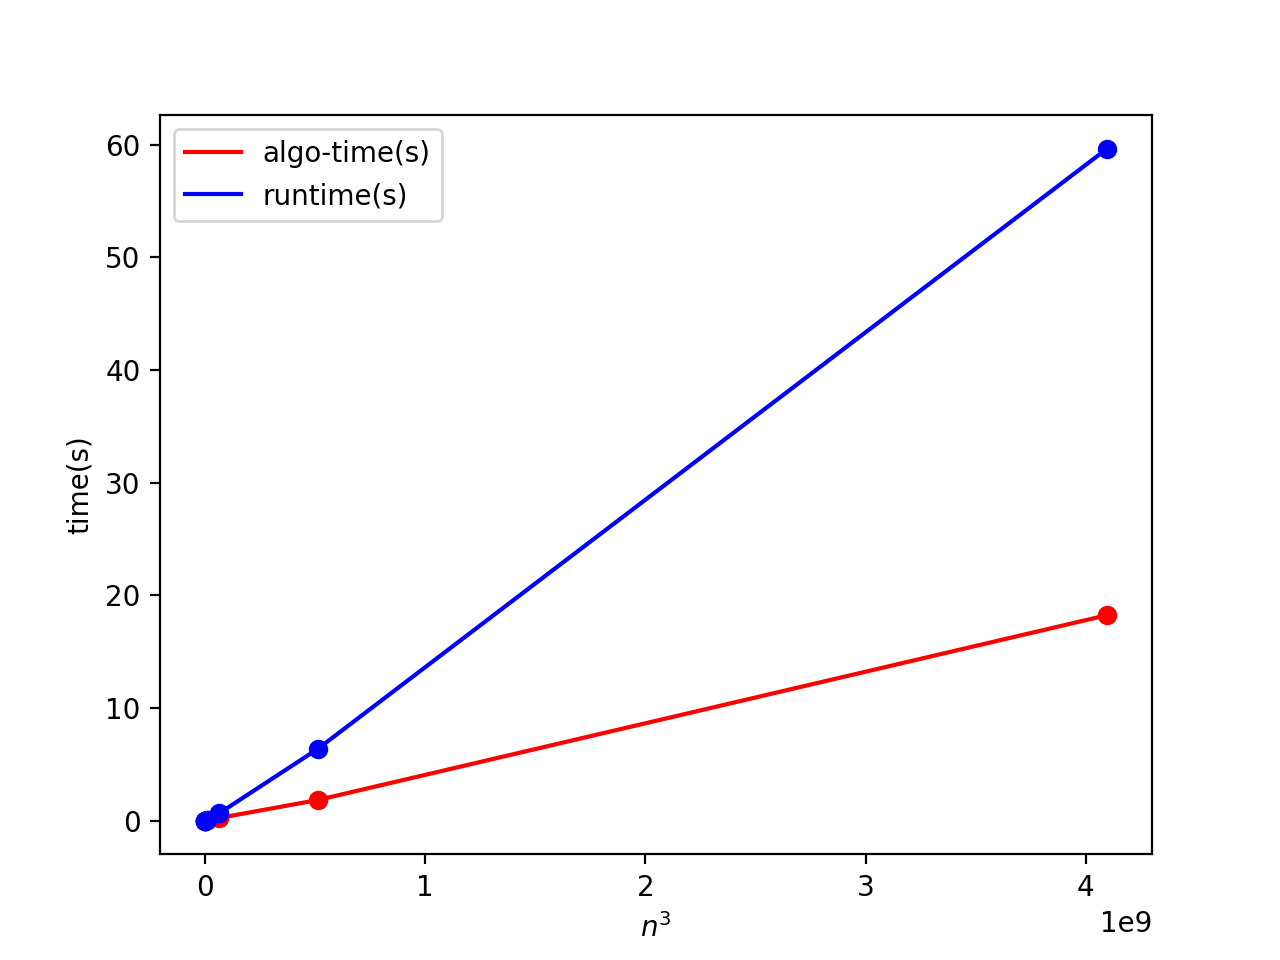
\includegraphics[width=0.75\textwidth]{src/algo2-runtime.png}
    \label{fig:algo2-runtime}
\end{figure}

\subsection{Algorithm-3 performance}
% Table generated by Excel2LaTeX from sheet '工作表1'
Table [\ref{tab:algo3}] shows detail results of Algorithm-3.
\begin{table}[htbp]
    \centering
    \caption{Algorithm-3 performance}
    \begin{tabular}{|c|c|c|c|c|}
        \hline
        \textbf{algo3} & \multicolumn{1}{c|}{n} & \multicolumn{1}{c|}{sigma} & \multicolumn{1}{l|}{algo-time(s)} & \multicolumn{1}{c|}{runrime(s)} \bigstrut\\
        \hline
        m3  & 3   & 7.87E-15 & 1.91E-06 & 0.004 \bigstrut\\
        \hline
        m4  & 10  & 7.83E-15 & 3.60E-05 & 0.015 \bigstrut\\
        \hline
        m5  & 100 & 1.86E-13 & 0.00776792 & 0.02 \bigstrut\\
        \hline
        m6  & 200 & 6.35E-13 & 0.022558 & 0.094 \bigstrut\\
        \hline
        m7  & 400 & 2.32E-12 & 0.164832 & 0.586 \bigstrut\\
        \hline
        m8  & 800 & 8.79E-12 & 1.33471 & 5.788 \bigstrut\\
        \hline
        m9  & 1600 & 3.45E-11 & 10.458 & 50.275 \bigstrut\\
        \hline
    \end{tabular}%
    \label{tab:algo3}
\end{table}%
\subsubsection{Sigma}
From Table [\ref{tab:algo3}], we can found that sigma in algorithm-2 and algoritm-3 is almost same, so they have the same accuracy.
\subsubsection{runtime to $n^3$}
\begin{figure}[H]
    \centering
    \caption{runtime to $n^3$}
    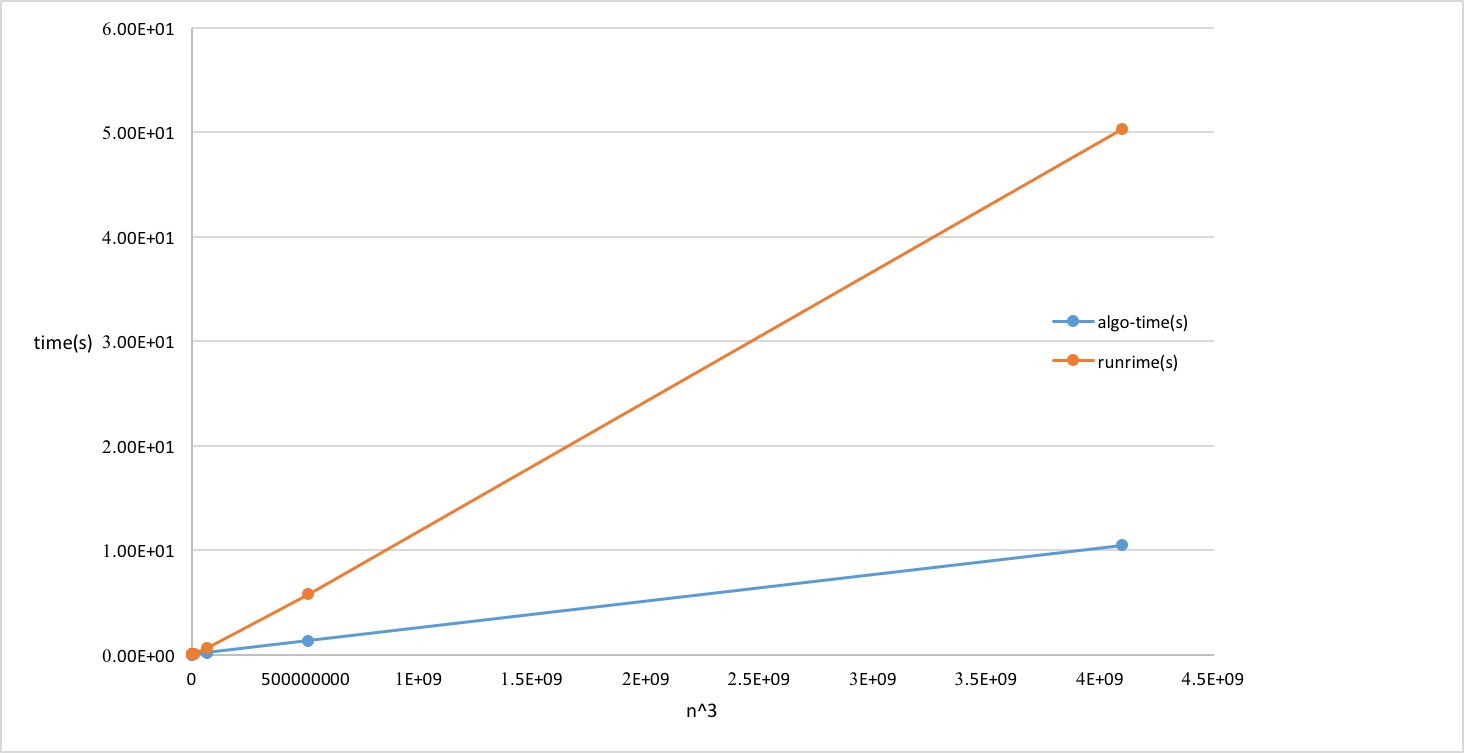
\includegraphics[width=0.75\textwidth]{src/algo3-runtime.png}
    \label{fig:algo3-runtime}
\end{figure}

\subsection{Comparison}
\subsubsection{Accuracy}
From Section \ref{sec:algo1-sigma}, we can found that Algorithm-1 is the worst method for \textbf{Gram-Schmidt process} because it is not
quite accurate. However, Algorithm-2 and Algorithm-3 almost have the same accuracy.
\subsubsection{Speed}
From Table [\ref{tab:algo2}] and Table [\ref{tab:algo3}], we found that both algo-time and runtime consumed by Algorithm-3 are a little
smaller than Algorithm-2, so Algorithm-3 is faster than Algorithm-2.
\subsubsection{Data transfer}
From Table [\ref{tab:algo1}][\ref{tab:algo2}][\ref{tab:algo3}], we can see that algo-time only takes about $\frac{1}{4}$ of total
execution time; in other words, dimension of matrix in \textbf{mX.dat} may also play an important role in this homework.

%\begin{align*}
%    & G_1  = A_1; \\
%    & \mbox{for (k = 2 ..... n)\{} \\
%    & \hspace{2em}G_k = 0; \\
%    & \hspace{2em} \mbox{for (i = 1 .... k-1)\{} \\
%    & \hspace{4em} G_k += ((A^T_kG_i)G_i) / (G^T_iG_i); \\
%    & \hspace{2em} \} \\
%    & \hspace{2em} G_k = A_k - G_k \\
%    & \}
%\end{align*}

\end{document}
